%!TEX root = main.tex

\begin{figure*}[t!]
\centering
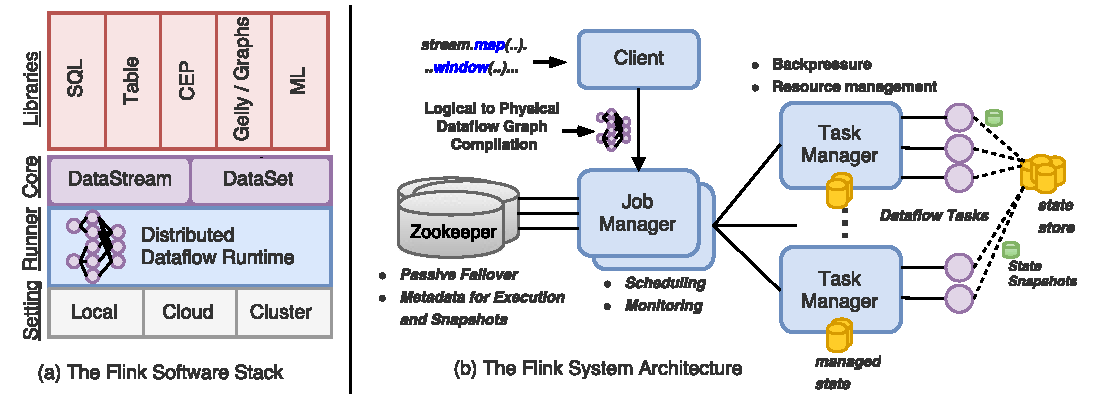
\includegraphics[width=\textwidth]{figures/flinkoverview.pdf}
\caption{An Overview of the Apache Flink System Model and Architecture.} 
\label{fig:flink-overview}
\vspace{-4mm}
\end{figure*}

\section{Background}

\subsection{The Apache Flink System}

The Apache Flink system \cite{CUSTOM:web/Flink} is an open-source project that provides a full software stack for programming, compiling and running distributed continuous data processing pipelines (\autoref{fig:flink-overview}(a)). Pipelines can be written as a series of data-centric transformations expressed in a fluid, functional programming API. At the core of the model there are two basic abstract data types, the \emph{DataSet} and \emph{DataStream} representations which target bounded and unbounded datasets respectively. Computation declared using high-level domain-specific libraries such as the SQL and Machine Learning (ML) packages, in fact, translates into a logical pipeline using these core representations. A major distinctive trait of the Flink programming model is the capability to declare local or partitioned application state within continuous user-defined transformations through managed data collections with diverse properties (append-only, mutable, etc.). Flink's runtime ensures that consistency is guaranteed for any managed state declared despite potential partial failures or reconfiguration periods.

Logical pipeline representations are optimised and mapped to physical graphs of dataflow operators encapsulating the user-defined logic at the client side. Physical graph representations are shipped to Flink's runtime, a continuous dataflow execution environment which deploys and manages their continuous execution as depicted in \autoref{fig:flink-overview}(b). As with most distributed data processing systems, there is a \emph{JobManager}, a master process that holds the metadata of active pipelines and coordinates execution by communicating with worker processes, the TaskManagers. Communication between the the JobManager and TaskManagers respects an asynchronous RPC-based communication protocol, consisting of periodic status updates (heartbeats) to the JobManager and scheduling requests back to the TaskManagers. In contrast to batch-centric job management \cite{zaharia2012discretized,venkataramandrizzle} which prioritizes reconfiguration and coordination, Flink employs a schedule-once, long-running allocation of tasks. However, the system is flexible to trivially reconfigure pipelines to more or less workers and re-allocate application state on-demand. This approach minimizes management overhead while allowing for fast adaptation to hardware or software changes or partial failures that can potentially occur. Finally, pipeline deployments in Flink are highly available, thus, tolerating both master and worker failures via leader election and passive failover in Zookeeper. All underlying mechanisms for state partitioning, snapshotting and maintenance are the main focus and covered throughly in this paper.


\subsection{Snapshots and Rollback Recovery}
\paris{It is a good chance here to explain what is exactly-once etc. and link them to snapshot properties. This is probably the only mildy theoretical part but it needs to be so just enough to help non-pro folks to understand the concepts we are covering}